\chapter{Υλικά και Μέθοδοι}

Σε αυτή την ενότητα θα περιγράψουμε μια μια τις διαδικασίες που ακολουθήσαμε ώστε να παράξουμε τα επιθυμητά αποτελέσματα. Αρχικά θα περιγράψουμε το σύστημα καταγραφής της κίνησης που υλοποιήθηκε. Στην συνέχεια θα εξηγήσουμε το πως κατασκευάσαμε το μοντέλο μας και το τι δυνατότητες έχει. Έπειτα θα περάσουμε στο κομμάτι της ανάλυσης, ξεκινώντας με το πρόβλημα της αντίστροφης κινηματικής και θα περιγράψουμε δυο απαραίτητες διαδικασίες ώστε να επιτευχθεί ορθό αποτέλεσμα με βάση την καταγεγραμμένη κίνηση. Στην συνέχεια χρησιμοποιώντας το αποτέλεσμα της αντίστροφης κινηματικής ήμαστε σε θέση να επιλέξουμε ανάμεσα σε δυο διαφορετικές τεχνικές εύρεσης των ροπών και δυνάμεων στο μοντέλο. Αρχικά θα περιγράψουμε μέθοδο της αντίστροφης δυναμικής και στην συνέχεια της ορθής δυναμικής και θα εξηγήσουμε πως τις χρησιμοποιήσαμε στις αναλύσεις μας, δίνοντας παράδειγμα στις μεθόδους που έγιναν χρήση. Θα αναφερθεί η μέθοδος εύρεσης των μυϊκών διεγέρσεων είτε μέσω της αντίστροφης δυναμικής σε συνδυασμό με την στατική βελτιστοποίηση, είτε με χρήση της ορθής δυναμικής και χρήση της στατικής βελτιστοποίησης σε κλειστό βρόγχο.

%Σε αυτή την ενότητα θα περιγράψουμε την διαδικασία με την οποία συλλέχθηκαν τα δεδομένα αλλά και την πορεία της επεξεργασίας τους ώστε να εξαχθούν τα επιθυμητά αποτελέσματα. Όπως φαίνεται στην εικόνα \ref{fig:methods-process1} αρχικά συλλέγονται τα δεδομένα με την βοήθεια της συσκευής \eng{Kinect}, αλλά και των εξωτερικών δυνάμεων αν είναι υπαρκτές. Τα δεδομένα αυτά προτού επεξεργαστούν στα μετέπειτα στάδια φιλτράρονται κατάλληλα, ώστε να μειωθούν οι ανεπιθύμητες παρεμβολές του θορύβου. Έπειτα ακολουθεί η διαδικασία της αντίστροφης κινηματικής, που με την βοήθεια ενός μοντέλου εξάγονται οι γενικευμένες συντεταγμένες (γωνίες) στις αρθρώσεις. Με χρήση αριθμητικών μεθόδων παραγωγίζουμε δύο φορές το αποτέλεσμα, ώστε να έχουμε στην διάθεση μας τις γενικευμένες ταχύτητες και επιταχύνσεις των αρθρώσεων του μοντέλου. Εφαρμόζουμε αντίστροφη δυναμική και εξάγουμε τις γενικευμένες ροπές στις αρθρώσεις που απαιτούνται για να παράξουν την δοσμένη κίνηση. Τέλος, έχοντας προσδώσει τους κατάλληλους μύες στο μοντέλο με βάση την γεωμετρία, αλλά και της δυναμικής τους μπορούν να εκτιμηθούν οι δυνάμεις που ασκεί ο κάθε μυς.
%

%%%%%%%%%%%%%%%%%%%%%%%%%%%%%%%%%%%%%%%%%%%%%%%%%%%%%%%%%%%%%%%%%%%%%%%%%%%%%%%%
\section{Καταγραφή της Κίνησης}

Όπως αναφέραμε χρησιμοποιούμε το \eng{Kinect} για την συλλογή των τροχιών των αρθρώσεων για μια δοσμένη κίνηση. Για την ανίχνευση του σκελετού εκμεταλλευόμαστε τον αλγόριθμο που είναι υλοποιημένος εσωτερικά στην συσκευή και έχουμε στην διάθεση μας στις τρισδιάστατες συντεταγμένες των αρθρώσεων. Το λογισμικό που χρησιμοποιείται για την καταγραφή της κίνησης έχει υλοποιηθεί στην \eng{C++} και βασίζεται στην βιβλιοθήκη της \eng{Microsoft} για το \eng{Kinect} (\eng{Microsoft Kinect SDK}). Επιπλέον γίνεται χρήση φίλτρων για την εξομάλυνση της κίνηση και την απαλοιφή του θορύβου λόγω \eng{jitter}. Τα αποτελέσματα μπορούν να καταγραφούν σε διαφορετικούς τύπους αρχείων, ώστε να χρησιμοποιηθούν στα μετέπειτα στάδια της ανάλυσης.

Το πρόγραμμα καταγραφής που υλοποιήθηκε έχει σαν στόχο την καταγραφή της χρονικής μεταβολής των θέσεων των αρθρώσεων και την βελτίωση των μετρήσεων. Για να ελαχιστοποιηθούν οι καθυστερήσεις και να μην ελαττωθεί ο ρυθμός επεξεργασίας των πακέτων που εισέρχονται από το \eng{Kinect}, έχουν ενεργοποιηθεί μόνο οι δυνατότητες παρακολούθησης του σκελετού και την πρόσληψη έγχρωμου βίντεο, για να μπορούμε να αντιληφθούμε το ορατό πεδίο του αισθητήρα όπως φαίνεται στην εικόνα \ref{fig:motion-capture}.

\begin{figure}[H]
    \centering
    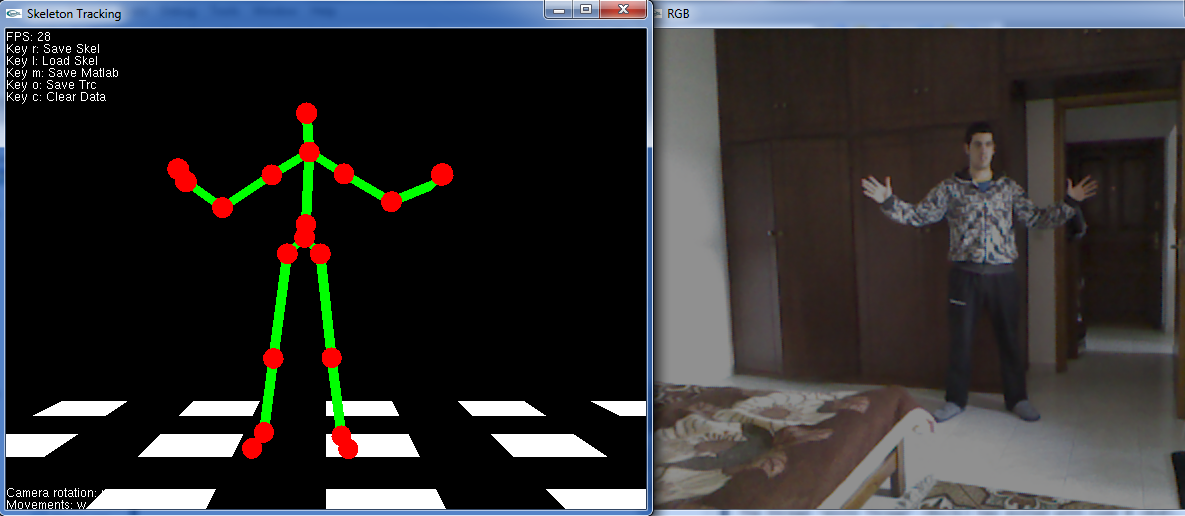
\includegraphics[width=.9\textwidth, keepaspectratio]{fig/motion-capture.png}
    \caption{Επίδειξη του συστήματος καταγραφής της κίνησης που υλοποιήθηκε}
    \label{fig:motion-capture}
\end{figure}

Πρέπει να σημειωθεί ότι η υλοποίηση έγινε με χρήση της βιβλιοθήκη \eng{OpenGL}. Υπάρχουν δύο παράθυρα, όπου στο ένα αναπαριστάται η τελευταία ακολουθία θέσεων του σκελετού, ενώ στο άλλο γίνεται αποτύπωση της έγχρωμης εικόνας που λαμβάνουμε ανά τακτικά χρονικά διαστήματα σαν εικόνα υφής, με αποτέλεσμα να έχουμε μια ανανέωση του περιεχομένου (δηλαδή βίντεο). Η περιήγηση στο τρισδιάστατο χώρο του αριστερού παραθύρου μπορεί να γίνει με την βοήθεια του ποντικιού και του πληκτρολογίου, δίνοντας την δυνατότητα αναπαράστασης του μοντέλου από διαφορετικές οπτικές γωνίες.

Εσωτερικά αποθηκεύονται οι παρελθοντικές τιμές των θέσεων σε ειδικές δομές μαζί με όλη την πληροφορία που διαθέτει το \eng{Kinect}. Παρέχεται η δυνατότητα αποθήκευσης των δεδομένων σε δυαδική, μορφή η οποία είναι εύκολη στην ανάγνωση και δεν απαιτεί υλοποίηση πολύπλοκων συναρτήσεων ανάγνωσης. Επίσης υπάρχουν επιλογές για αποθήκευση των τροχιών σε μορφή \lq \eng{.dat}\rq\; της \eng{Matlab} και σε μορφή \lq \eng{.trc}\rq  , που είναι συμβατή με το εργαλείο \eng{OpenSim}.

Όπως φαίνεται και στο διάγραμμα κλάσεων \ref{fig:motion-capture-class-diagram}, η κλάση \eng{Kinect} υλοποιεί την διασύνδεση με τον αισθητήρα και αναλαμβάνει να επεξεργάζεται τα δεδομένα που εισέρχονται από το \eng{Kinect}. Όταν έρθουν πακέτα από την έγχρωμη κάμερα απλά γεμίζει τον πίνακα \eng{rgbStream} με τις τιμές των αντίστοιχων χρωμάτων, που στην συνέχει αποτυπώνονται από την μηχανή αναπαράστασης. Όταν έρθουν δεδομένα που αφορούν τον σκελετό, αρχικά φιλτράρονται με το προεπιλεγμένο φίλτρο και έπειτα τα δεδομένα συγκρατούνται από την κλάση \eng{Skeleton} μαζί με την χρονική στιγμή της άφιξης τους. Η κλάση \eng{Skeleton} συγκρατεί την χρονική ακολουθία των δεδομένων του σκελετού. Επίσης είναι σε θέση να το αναπαραστήσει σε συνδυασμό με την μηχανή αναπαράστασης, αλλά υπάρχει και η δυνατότητα αποθήκευσης των αποτελεσμάτων της κίνησης σε διάφορες μορφές, ώστε να χρησιμοποιηθούν για ανάλυση. Η κλάση \eng{Viewer} είναι η μηχανή αναπαράστασης που αναλαμβάνει να σχεδιάσει τον σκελετό και την έγχρωμη εικόνα, δίνοντας την δυνατότητα περιήγησης στο τρισδιάστατο χώρο, αλλά και αλληλεπίδρασης με τον χρήστη, έχοντας κάποιες προεπιλεγμένες εντολές που αναγράφονται στο παράθυρο. Τέλος, υπάρχει η δυνατότητα αλλαγής κάποιων παραμέτρων μέσω του αρχείου \eng{settings.ini}, όπως είναι ο τρόπος φιλτραρίσματος, οι ονομασίες των ενδείξεων (\eng{markers}), η τοποθεσία και το όνομα των αρχείων που αποθηκεύονται και η δυνατότητα ρύθμισης \eng{timer}, ώστε να συλλεχθούν τα δεδομένα αυτόματα μετά από μια χρονική στιγμή.

\begin{figure}[H]
    \centering
    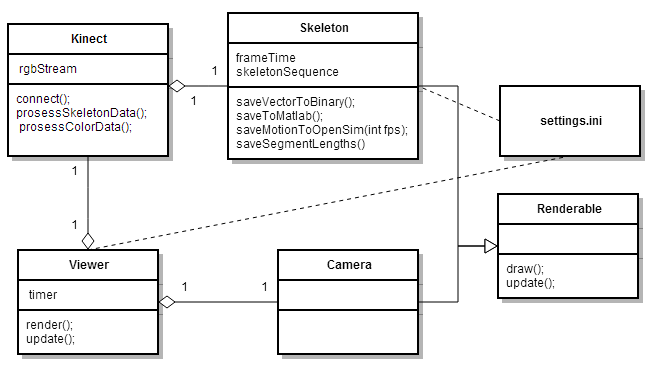
\includegraphics[width=.9\textwidth, keepaspectratio]{fig/motion-capture-class-diagram.png}
    \caption{Διάγραμμα κλάσεων για το πρόγραμμα καταγραφής}
    \label{fig:motion-capture-class-diagram}
\end{figure}

%%%%%%%%%%%%%%%%%%%%%%%%%%%%%%%%%%%%%%%%%%%%%%%%%%%%%%%%%%%%%%%%%%%%%%%%%%%%%%%%
\section{Δημιουργία του Μοντέλου}

Πριν περιγράψουμε την διαδικασία της δημιουργίας του μοντέλου θα ήθελα να αναφερθώ στα εργαλεία που χρησιμοποιήθηκαν. Για την μοντελοποίηση αλλά και την διεξαγωγή των αναλύσεων χρησιμοποιήθηκε το ανοιχτό εργαλείο-βιβλιοθήκη \eng{OpenSim}. Το \eng{OpenSim} είναι μια πλατφόρμα που βασίζεται στην μηχανή \eng{SimTK Simbody} για την μοντελοποίηση, προσομοίωση και ανάλυση νευρομυοσκελετικών συστημάτων \cite{delp07}. Το εργαλείο διαθέτει γραφική διεπαφή, αλλά και διεπαφή για τον προγραμματιστή σε γλώσσα \eng{C++}. Είναι δυνατή η επέκταση του λογισμικού με την βοήθεια \eng{plugins}. Το \eng{OpenSim} χρησιμοποιείται ευρέως από την επιστημονική κοινότητα κυρίως σε βιοϊατρικές εφαρμογές. Η κοινότητα διαθέτει μεγάλο αριθμό από έτοιμα μοντέλα, πειραματικά δεδομένα και επιπρόσθετα εργαλεία για την διεξαγωγή των αναλύσεων.

\begin{figure}[H]
    \centering
    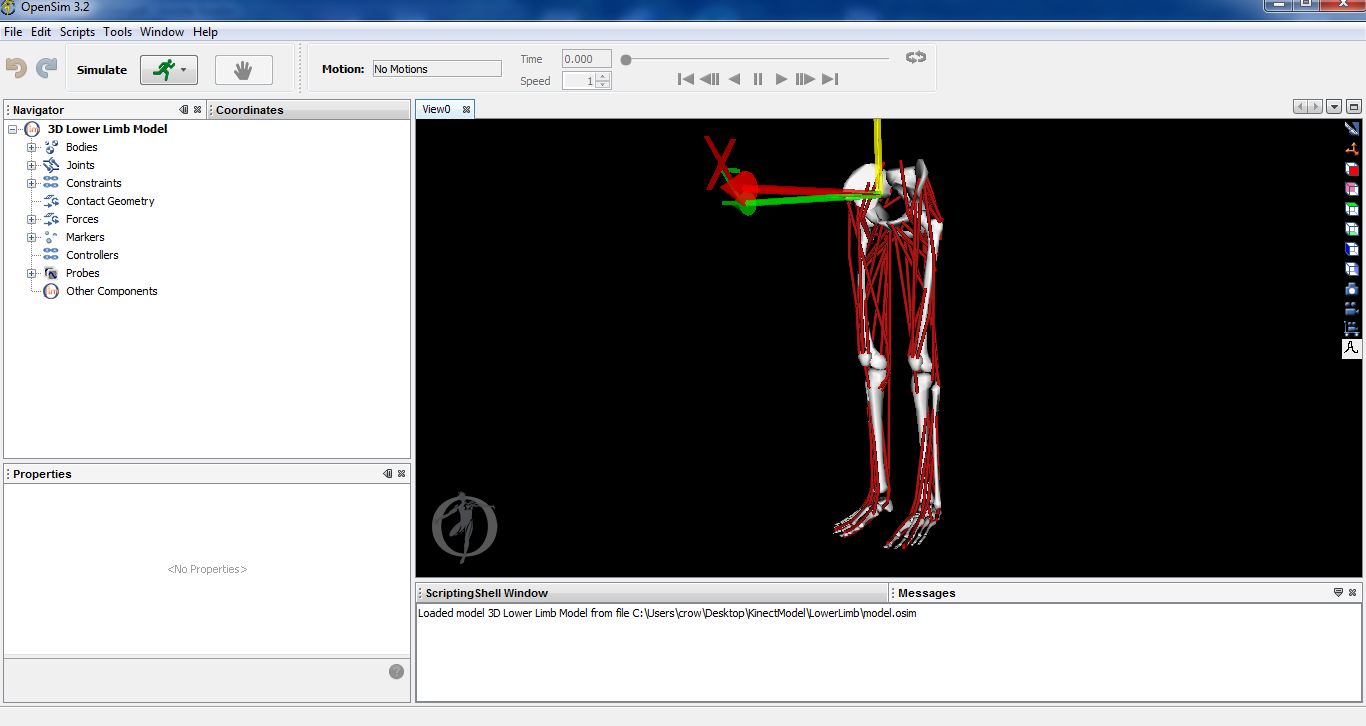
\includegraphics[width=0.8\textwidth, keepaspectratio]{fig/opensim.png}
    \caption{Γραφική διεπαφή του \eng{OpenSim}}
    \label{fig:opensim-gui}
\end{figure}

Δεν θα μπορούσα να παραλείψω βέβαια και το \eng{Simbody}, το οποίο είναι η καρδιά της πλατφόρμας. Σαν μηχανή φυσικής, δίνει την δυνατότητα περιγραφής πολύπλοκων διατάξεων με έναν μεγάλο αριθμό από έτοιμα στοιχεία όπως είναι η μοντελοποίηση δυνάμενων, εισαγωγή περιορισμών στην κίνηση, περιγραφή της διάταξης, ποικίλα τύπων βαθμών ελευθερίας και άλλα πολλά. Έχει σχεδιαστεί κατάλληλα ώστε να ωθεί την αποδοτικότητα και παράλληλα να μην μειώνει την ευελιξία. Είναι ένα εργαλείο που σου δίνει την δυνατότητα να περιγράφεις και να προσομοιώσεις τα φαινόμενα που μελετάς.

%Όσον αφορά τις δυνατότητες που προσφέρει η προγραμματιστική βιβλιοθήκη του \eng{OpenSim} μπορούμε να διακρίνουμε κάποια βασικά χαρακτηριστικά \ref{fig:opensim-architecture}. Βλέπουμε ότι στην βάση βρίσκεται το \eng{Simbody}. Επιπλέον έχει δοθεί η δυνατότητα περιγραφής του μοντέλου και επιπρόσθετα στοιχεία που βοηθούν στο να γίνει η ανάλυση. Το \eng{OpenSim} βοηθάει στο να γίνει η περιγραφής της σκελετικής διάταξης, να προδοθούν βαθμοί ελευθερίας και περιορισμοί στην κίνηση. Ακόμη υπάρχει η δυνατότητα μοντελοποίησης των μυών και η προσθήκη τους στην διάταξη. Όπως θα δούμε και στην συνέχει μπορούν να εξαχθούν πληθώρα είδη αναλύσεων που μπορούν να χρησιμοποιηθούν από τους αναλυτές.
%
%\begin{figure}[H]
%    \centering
%    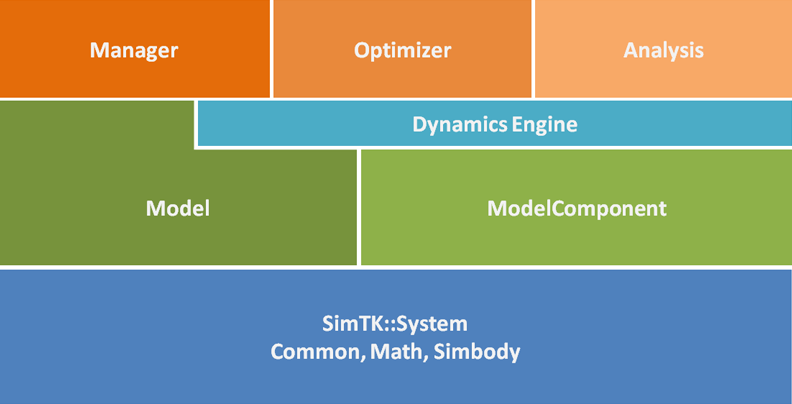
\includegraphics[width=0.8\textwidth, keepaspectratio]{fig/opensim-architecture.png}
%    \caption{Συνοπτική αρχιτεκτονική της βιβλιοθήκης του \eng{OpenSim}\protect\footnotemark}
%    \label{fig:opensim-architecture}
%\end{figure}
%\footnotetext{Εικόνα από την ιστοσελίδα \eng{\url{http://simtk-confluence.stanford.edu:8080/display/OpenSim/The+OpenSim+API}}}

%%%%%%%%%%%%%%%%%%%%%%%%%%%%%%%%%%%%%%%%%%%%%%%%%%%%%%%%%%%%%%%%%%%%%%%%%%%%%%%%
\subsection{Επεξήγηση του Μοντέλου}

Για την διεξαγωγή των προσομοιώσεων είναι αναγκαία η σχεδίαση ενός μοντέλου που θα είναι όσο το δυνατόν πιο αντιπροσωπευτικό σε σχέση με το πραγματικό. Η διαδικασία είναι πολύπλοκη και απαιτεί γνώσεις όχι μόνο της φυσιολογίας του ανθρώπου, αλλά και γνώσεις για να περιγραφεί η λειτουργία του μοντέλου. Στην παρούσα μελέτη έχει μοντελοποιηθεί το τμήμα των κάτω άκρων του ανθρώπου, ώστε να γίνει η μελέτη κατά την διεξαγωγή κινήσεων βαδίσματος.

Το μοντέλο αποτελείται από 20 βαθμούς ελευθερίας, από τους οποίους οι 6 έχουν να κάνουν με τον προσανατολισμού και την περιστροφή της λεκάνης που είναι και η ρίζα της ιεραρχίας. Οι υπόλοιποι 7 βαθμούς ελευθερίας για κάθε πόδι. Επίσης το μοντέλο διαθέτει 43 μύες τύπου \eng{Hill} για κάθε πόδι, που βασίζονται στο πρόσφατο μοντέλο \eng{millard13}, οι οποίοι είναι τοποθετημένοι με βάση την πραγματική τους γεωμετρία γύρω από τα οστά. Οι μύες είναι σε θέση να παράξουν έργο στις αντίστοιχες αρθρώσεις, ώστε να δημιουργηθεί η επιθυμητή κίνηση. Επίσης λόγω της έλλειψης δεδομένων που αφορούν τις εξωτερικές δυνάμεις αντίδρασης από το δάπεδο κατά την κίνηση, έχει γίνει η κατάλληλη μοντελοποίηση τους με χρήση δυνάμεων επαφής. Το μοντέλο έχει δημιουργηθεί στα πλαίσια μελέτης πως μπορεί μια εγχείρηση να αλλάξει τις παραμέτρους των μυών και κατά συνέπεια το αποτέλεσμα της βάδισης με βάση το \cite{delp90} και τροποποιήθηκε κατάλληλα στην παρούσα εργασία.

\begin{figure}[H]
    \centering
    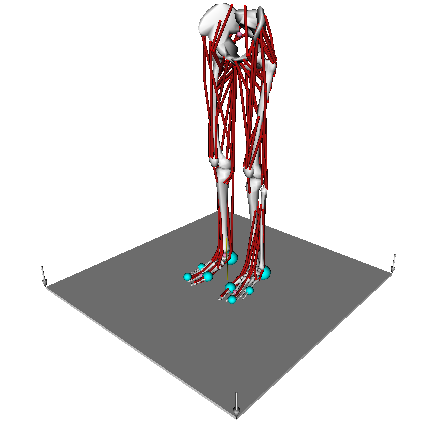
\includegraphics[height=0.38\textheight, keepaspectratio]{fig/lower-limb-model.png}
    \caption{Μυοσκελετικό μοντέλο με το δάπεδο αντίδρασης}
    \label{fig:lower-limb-model}
\end{figure}

\begin{center}
    \begin{tabular}{ccc}
        \toprule
        % after \\: \hline or \cline{col1-col2} \cline{col3-col4} ...
        Άρθρωση & Κάτω όριο & Πάνω όριο\\
        \midrule
        \eng{pelvis\_till (z)} & $-90^{o}$ & $+90^{o}$\\
        \eng{pelvis\_list (x)} & $-90^{o}$ & $+90^{o}$\\
        \eng{pelvis\_rotation (y)} & $-90^{o}$ & $+90^{o}$\\
        \eng{pelvis\_tx} & $-5$ & $+5$\\
        \eng{pelvis\_ty} & $-1$ & $+2$\\
        \eng{pelvis\_tz} & $-3$ & $+3$\\
        \eng{hip\_flexion} & $-95^{o}$ & $+95^{o}$\\
        \eng{hip\_adduction} & $-50^{o}$ & $+15^{o}$\\
        \eng{hip\_rotation} & $-20^{o}$ & $+20^{o}$\\
        \eng{knee\_angle} & $-120^{o}$ & $+0^{o}$\\
        \eng{ankle\_angle} & $-30^{o}$ & $+30^{o}$\\
        \eng{subtalar\_angle} & $-20^{o}$ & $+20^{o}$\\
        \eng{mtp\_angle} & $-30^{o}$ & $+30^{o}$\\
        \bottomrule
    \end{tabular}
    \captionof{table}{Βαθμοί ελευθερίας με τους αντίστοιχους περιορισμούς}
    \label{tab:model-dof}
\end{center}

Όπως φαίνεται και στον πίνακα \ref{tab:model-dof} παρουσιάζονται οι βαθμοί ελευθερίας του μοντέλου μαζί με τους περιορισμούς στην επιτρεπτή κίνηση. Ο γοφός έχει τρεις περιστροφικούς βαθμούς, το γόνατο έναν, ο αστράγαλος δύο και τα δάχτυλα των ποδιών έναν. Η λεκάνη φροντίζει να προσανατολίσει και να τοποθετήσει κατάλληλα το μοντέλο στο χώρο και στην πραγματικότητα δεν συνδέεται με κάποια βιολογική λειτουργία. Αυτός ο πλεονασμός της λεκάνη είναι μια από της τροποποιήσεις του αρχικού μοντέλου ώστε να μπορεί να βρεθεί το μοντέλο σε διαφορετικές διατάξεις στον χώρο.

Η έλλειψη εξωτερικών δυνάμεων αντίδρασης από το δάπεδο είναι σοβαρό μειονέκτημα που οδηγεί σε προσεγγίσεις της πραγματικότητας. Στις αναλύσεις χρησιμοποιήθηκαν δεδομένα τα οποία πάρθηκαν από τρίτους και περιείχαν την μέτρηση της αντίδρασης εδάφους. Ωστόσο έγινε μια προσπάθεια ενσωμάτωση και εκτίμηση των δυνάμεων επαφής με το δάπεδο \cite{seitha11}. Το \eng{OpenSim} χρησιμοποιεί δύο τύπων δυνάμεων επαφής που έχουν υλοποιηθεί από το \eng{Simbody}. Η πρώτη είναι η \eng{Hunt Crossley Force} που βασίζεται στην θεωρία επαφής του \eng{Hertz} \cite{hunt75}. Αυτή η μέθοδος υπολογίζει την ελαστική παραμόρφωση αναλυτικά και το \eng{Simbody} υποστηρίζει κάποια βασικά γεωμετρικά σχήματα. Στην μοντελοποίηση που κάναμε έχει χρησιμοποιηθεί μια επιφάνεια για το δάπεδο και έχουν τοποθετηθεί σφαίρες στις πατούσες. Η εναλλακτική λύση είναι η αναπαράσταση της γεωμετρίας με πλέγματα (\eng{mesh}) τα οποία αποτελούνται από ελατήρια για την μοντελοποίηση της ελαστικότητας \cite{hertz82}. 

Παρόλο της μεγάλης προσπάθειας τα αποτελέσματα με χρήση μοντέλων εκτίμησης της αντίδρασης εδάφους δεν έδωσαν βιολογικά ορθά αποτελέσματα κατά την βάδιση γιατί παράλληλα απαιτούν βαθμονόμιση για να μπορούν να λειτουργούν και να δώσουν ικανοποιητική λύση. Η αιτία είναι σε προβλήματα εκτίμησης της διάταξης του ποδιού από τον αισθητήρα που εκτιμούσε λανθασμένα τον προσανατολισμό. Με αποτέλεσμα το πόδι κάνει σωστή επαφή με το έδαφος και να μην εκτιμάται σωστά οι δυνάμεις αντίδρασης καθιστώντας την ανάλυση ασταθή. Αυτό είναι δύσκολο κατά την εκτέλεση της βάδισης, ωστόσο για απλές εκτιμήσεις όπως είναι η ρίψη του μοντέλου από κάποιο ύψος και η εξέταση ποιες δυνάμεις θα ασκηθούν κατά την σύγκρουση με το έδαφος τα αποτελέσματα είναι ορθά. 

\begin{figure}[H]
    \centering
    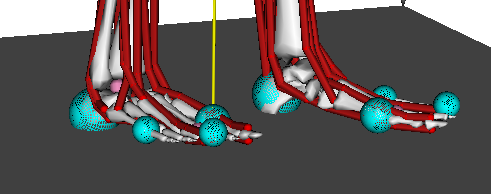
\includegraphics[width=0.8\textwidth, keepaspectratio]{fig/foot-contact.png}
    \caption{Συνοπτική αναπαράσταση των σφαιρών ελαστικότητας στα πόδια}
    \label{fig:foot-contact}
\end{figure}

Όσον αφορά τους μύες, έχουν τροποποιηθεί ώστε να χρησιμοποιούν το έτοιμο μοντέλο μυ \eng{Millard2013EquilibriumMuscle} που είναι υλοποιημένο στην βιβλιοθήκη του \eng{OpenSim}. Οι παράμετροι των μυών (μέγιστη παραγόμενη δύναμη, βέλτιστο μήκος μυ, μήκος χαλαρότητας του τένοντα, σχετική γωνία μεταξύ μυ και τένοντα, γεωμετρία) έχουν προσδιοριστεί από το αρχικό μοντέλο και είναι συμβατά με το νέο μοντέλο μυ.

%%%%%%%%%%%%%%%%%%%%%%%%%%%%%%%%%%%%%%%%%%%%%%%%%%%%%%%%%%%%%%%%%%%%%%%%%%%%%%%%
\section{Προετοιμασία για την Αντίστροφη Κινηματική}

Αφού έχει καταγραφεί μια κίνηση και υπάρχει το αντίστοιχο μοντέλο μπορεί να λυθεί το πρόβλημα της αντίστροφης κινηματικής ώστε να προσδιορισθούν οι γενικευμένες συντεταγμένες (συνήθως γωνίες) για την δοσμένη κίνηση. Προτού όμως εκτελέσουμε την αντίστροφη κινηματική πρέπει να γίνουν κάποια επιπλέον βήματα.

%%%%%%%%%%%%%%%%%%%%%%%%%%%%%%%%%%%%%%%%%%%%%%%%%%%%%%%%%%%%%%%%%%%%%%%%%%%%%%%%
\subsection{Τοποθέτηση Ενδείξεων}

\begin{figure}[H]
    \centering
    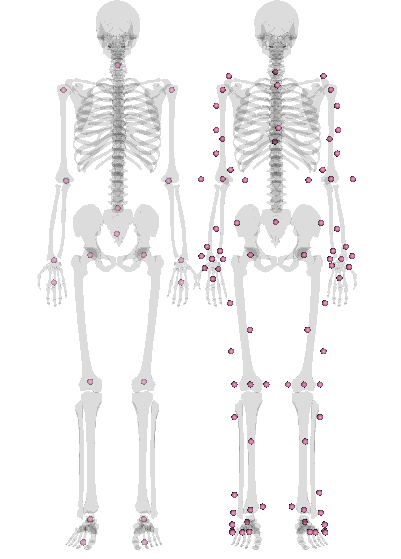
\includegraphics[height=0.6\textheight, keepaspectratio]{fig/kinect-vicon-markers.png}
    \caption{Σύγκριση συστήματος ενδείξεων του \eng{Kinect} και του \eng{Vicon} δεξιά}
    \label{fig:kinect-vicon-markers}
\end{figure}

Αρχικά πρέπει να προσδιοριστούν οι αντιστοιχίες μεταξύ της καταγεγραμμένης κίνησης και του μοντέλου. Ωστόσο μην ξεχνάμε ότι το πρόβλημα της αντίστροφης κινηματικής προσπαθεί να βρει τις γωνίες που πρέπει να τροφοδοτήσει το μοντέλο ώστε να ταιριάξει με την δοσμένη διάταξη της κίνησης. Αφού τα πειράματα έγινα με την βοήθεια του \eng{Kinect}, έχουμε στην διάθεση μας τις θέσεις των αρθρώσεων. Συνεπώς, πρέπει να τοποθετηθούν οι αντίστοιχες ενδείξεις στις αρθρώσεις του μοντέλου.

Στην εικόνα \ref{fig:kinect-vicon-markers} με ροζ χρώμα συμβολίζεται οι ενδείξεις (\eng{marker}). Από αριστερά βλέπουμε τις ενδείξεις που απαιτούνται για να συνδεθεί η καταγεγραμμένη κίνηση από το \eng{Kinect}, ενώ από δεξιά βλέπουμε τους ενδείξεις που απαιτούνται για να γίνει μια καταγραφή από ένα επαγγελματικό σύστημα της εταιρίας \eng{Vicon}. Οι ενδείξεις προσδιορίζονται με βάση την εφαρμογή, ωστόσο λόγω του ότι ο προσανατολισμός και η θέση στο χώρο ενός τμήματος του σώματος όπως είναι τα οστά απαιτεί ώστε να βρεθεί μοναδική λύση τουλάχιστον τρία μη συνευθειακά σημεία σε κάθε τμήμα. Αυτός είναι και ο λόγος για τον οποίον ο δεξής σκελετός έχει πιο πολλές ενδείξεις. Αυτό είναι και ένα βασικό μειονέκτημα του συστήματος μας σε σχέση με επαγγελματικά συστήματα, δηλαδή για κάποιες κινήσεις μπορεί να μην βρεθεί ο σωστός προσανατολισμός. Ωστόσο για απλές κινήσεις το αποτέλεσμα και με υψηλό ρυθμό δειγματοληψίας της κίνησης η αντίστροφη κινηματική πειραματικά δίνει ικανοποιητικά αποτελέσματα.

%%%%%%%%%%%%%%%%%%%%%%%%%%%%%%%%%%%%%%%%%%%%%%%%%%%%%%%%%%%%%%%%%%%%%%%%%%%%%%%%
\subsection{Κανονικοποίηση του Μοντέλου}

Το τελευταίο πράγμα που πρέπει να γίνει είναι η κανονικοποίηση του γενικού μοντέλου που έχουμε στην διάθεση μας, ώστε να αρμόζει σε διαφορετικά σωματότυπα. Το \eng{OpenSim} διαθέτει δυνατότητα μετατροπής του μοντέλου, αλλά και την θέση των ενδείξεων από το γενικό στο ειδικό. Η διαδικασία είναι σχετικά απλή και βελτιώνει σημαντικά το τετραγωνικό σφάλμα της αντίστροφης κινηματικής. Με βάση τις ενδείξεις που έχουν τοποθετηθεί στο γενικό μοντέλο γίνεται μια ομαδοποίηση ζευγαριών που αντιπροσωπεύουν κάποιο τμήμα του σώματος (π.χ. η ένδειξη του γοφού και του γονάτου αντιστοιχεί στο μηριαίο οστό) και υπολογίζεται ο συντελεστής παραμόρφωσης με βάση του αντίστοιχου ζευγαριού από την πειραματική κίνηση. Στην συνέχεια παραμορφώνεται το μοντέλο ώστε να αρμόζει όσον το δυνατών καλύτερα στις πειραματικές μετρήσεις.

Έχει γίνει κατάλληλη επιλογή των τμημάτων και των ζευγαριών ενδείξεων ώστε να μεταβληθούν κατάλληλα όλα τα τμήματα του σώματος. Επίσης δίνεται η δυνατότητα να διατηρηθεί η μάζα του γενικού μοντέλου. Το γενικό μοντέλο αντιπροσωπευθεί άντρα ύψους 1.80\eng{cm} και βάρος 75\eng{kg}. Το κάτω τμήμα που έχει παρθεί ζυγίζει 41\eng{kg}. Η μάζα και η αδράνεια κάθε οστού έχει προσδιοριστεί για το γενικό μοντέλο και τροποποιείται ανάλογα με βάση τις μετρήσεις.

\begin{center}
    \begin{tabular}{ccc}
        \toprule
        Τμήμα του σώματος & 1η ένδειξη & 2η ένδειξη\\
        \midrule
        \eng{pelvis} & \eng{HIP\_RIGHT} & \eng{HIP\_LEFT}\\
        \eng{femru} & \eng{HIP} & \eng{KNEE}\\
        \eng{tibia} & \eng{KNEE} & \eng{ANKLE}\\
        \eng{calcn} & \eng{ANKLE} & \eng{FOOT}\\
        \bottomrule
    \end{tabular}
    \captionof{table}{Τμήματα του σώματος και τα ζευγάρια των ενδείξεων για τα κάτω άκρα}
    \label{tab:scale-pairs}
\end{center}

%%%%%%%%%%%%%%%%%%%%%%%%%%%%%%%%%%%%%%%%%%%%%%%%%%%%%%%%%%%%%%%%%%%%%%%%%%%%%%%%
\subsection{Διεξαγωγή της Αντίστροφης Κινηματικής}

Αφού έχουν γίνει τα παραπάνω πλέον μπορεί να εκτελεστεί η αντίστροφη κινηματική και να παραχθούν οι γωνίες που απαιτούνται για την παραγωγή της δοσμένης κίνησης από το μοντέλο. Το αποτέλεσμα την αντίστροφης κινηματικής είναι ζωτικής σημασίας για τα μετέπειτα στάδια της ανάλυσης. Οι υπολογισμένες γωνίες αν αναπαρασταθούν δεν θα πρέπει να έχουν απότομες μεταβολές από μια στιγμή σε άλλη, ώστε να μην παράγουν μη φυσιολογικές επιταχύνσεις και με αποτέλεσμα δυνάμεις. Κατά την εύρεση λύσεων υπάρχουν γωνίες για τις οποίες η διάταξη βρίσκεται σε απροσδιοριστία μορφή. Το τελευταίο μπορεί να αποφευχθεί αν εισαχθούν οι κατάλληλοι περιορισμοί στις κινήσεις της διάταξης αφότου έχει μελετηθεί εκ των προτέρων.

Κατά την διεξαγωγή της αντίστροφης κινηματικής μαζί με το κανονικοποιημένο μοντέλο τροφοδοτούμε και τις συντεταγμένες που έχουμε καταγράψει από το \eng{Kinect}, οι οποίες βρίσκονται σε κατάλληλη μορφή (*.\eng{trc}) που υποστηρίζεται από το \eng{OpenSim} και έχουν φιλτραριστεί κατάλληλα ώστε η κίνηση να είναι ομαλή.

%%%%%%%%%%%%%%%%%%%%%%%%%%%%%%%%%%%%%%%%%%%%%%%%%%%%%%%%%%%%%%%%%%%%%%%%%%%%%%%%
\section{Προσδιορισμός των Ροπών και των Δυνάμενων}

Αφού έχουμε στην διάθεση μας τα αποτελέσματα της αντίστροφης κινηματικής το επόμενο βήμα είναι ο προσδιορισμός των γενικευμένων ροπών στις αρθρώσεις του μοντέλου, αλλά και η εκτίμηση των δυνάμεων που συνεισφέρει ο κάθε μυς. Ας υπενθυμίσουμε την σχέση που περιγράψαμε \ref{equ:dynamics-equation}, η οποία αποτελεί την λύση του προβλήματος του προσδιορισμού των ροπών στις αρθρώσεις. Η διαδικασία ονομάζεται αντίστροφη δυναμική (\eng{inverse dynamics}) και είναι ρουτίνα στις κλινικές μελέτες του προσδιορισμού των δυνάμεων και των ροπών. Τα απαραίτητα στοιχεί είναι οι εξωτερικές δυνάμεις, το αποτέλεσμα από την αντίστροφη κινηματική, οι ταχύτητες και οι επιταχύνσεις που υπολογίζονται με αριθμητικές μεθόδους και η περιγραφή της κατανομής της μάζας τους σώματος.

\begin{figure}[H]
    \centering
    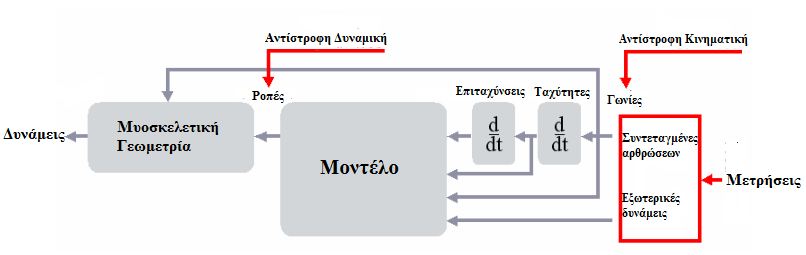
\includegraphics[width=0.8\textwidth, keepaspectratio]{fig/process.png}
    \caption{Διαδικασία εξαγωγής των δυνάμενων\protect\footnotemark}
    \label{fig:methods-process1}
\end{figure}
\footnotetext{Εικόνα από την ιστοσελίδα \eng{\url{http://simtk-confluence.stanford.edu:8080/display/OpenSim/Overview+of+the+OpenSim+Workflow}}}

Να τονίσουμε κάποια βασικά μειονεκτήματα της μεθόδου. Απαιτείται ο προσδιορισμός των εξωτερικών δυνάμεων που ασκούνται στην διάταξη, κάτι που δεν είναι πάντα διαθέσιμο. Επίσης η εκτίμηση της κατανομής της μάζας του ασθενή είναι ένα δύσκολο πρόβλημα και γίνονται προσεγγίσεις. Στην βιβλιογραφία υπάρχουν μέθοδοι που μετρώντας τα μήκη του σώματος μπορείς να εκτιμήσεις την μάζα τους, ωστόσο κατά την μοντελοποίηση της ροπής αδράνειας για λόγους απλότητας προσεγγίζονται τα τμήματα του σώματος με χρήση γνωστών γεωμετρικών σχημάτων. Όλες αυτές οι προσεγγίσεις οδηγούν σε συσσώρευση σφαλμάτων και την λάθος εκτίμηση των παραμέτρων κατά την κίνηση. Αν όμως αναζητούμε μια μεθόδους που παράγει αποτελέσματα γρήγορα και με ελάχιστο κόπο η αντίστροφη δυναμική είναι μια από αυτές.

Αν θα θέλαμε να υπολογίσουμε τις δυνάμεις των μυών πρέπει να συνδυάσουμε διαφορετικές τεχνικές που βασίζονται στην θεωρία της βελτιστοποίησης, αφού για μια δοσμένη κίνηση υπάρχουν πολλές λύσεις (δυνάμεις μυών) που μπορούν να παράξουν την κίνηση. Για το λόγο αυτό στην ανάλυση μπαίνουν κάποια κριτήρια που θα περιορίσουν τις επιτρεπτές λύσεις και θα παράξουν μια βέλτιστη με βάση αυτών. Στην βιβλιογραφία μια από αυτές τις τεχνικές είναι η στατική βελτιστοποίηση (\eng{static optimization}).

Ενώ η αντίστροφη δυναμική ξεκινά από το αποτέλεσμα της κίνησης και καταλήγει στο αίτιο που είναι οι ροπές στις αρθρώσεις, η ορθή δυναμική ξεκινά από το αίτιο που είναι η διέγερση του συστήματος και καταλήγει στην παραγωγή της κίνησης. Το αίτιο ανάλογα με το βάθος της ανάλυσης που επιθυμούμε θα μπορούσε να είναι και μια νευρική διέγερση από τον εγκέφαλο που καταλήγει σε παραγόμενη δύναμη από τους μύες που μετατρέπεται σε ροπή στις αρθρώσεις και συνεπώς σε κίνηση. Οι μέθοδοι που βασίζονται στην ορθή δυναμική είναι πιο ευέλικτες γιατί δεν απαιτείται άμεσα η γνώση των εξωτερικών δυνάμεων, ούτε των ροπών που ασκούνται στο σύστημα. Αυτές οι ποσότητες θα μπορούσαν να εκτιμηθούν με κάποιο κριτήριο. Για παράδειγμα η εκτίμηση της αντίδρασης του εδάφους θα μπορούσε να εκτιμηθεί αν μοντελοποιηθεί κατάλληλα και όταν πλησιάζει το πόδι στο έδαφος να ασκείται μια δύναμη ανάλογα με την απόσταση. Ωστόσο οι προσεγγίσεις αυτές οδηγούνται σε σφάλματα και δεν είναι πάντα βιολογικά σωστές. Από την άλλη η ροπές στις αρθρώσεις θα μπορούσαν να υπολογίζονται με κάποιο κριτήριο βελτιστοποίησης.

\begin{figure}[H]
    \centering
    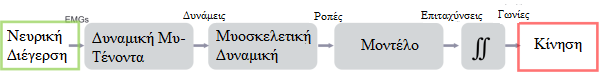
\includegraphics[width=1.0\textwidth, keepaspectratio]{fig/forward-simulation.png}
    \caption{Στάδια κατά την εκτέλεση της ορθής δυναμικής\protect\footnotemark}
    \label{fig:forward-simulation}
\end{figure}
\footnotetext{Εικόνα από την ιστοσελίδα \eng{\url{http://simtk-confluence.stanford.edu:8080/display/OpenSim/Overview+of+the+OpenSim+Workflow}}}

Όπως φαίνεται και στην εικόνα \ref{fig:forward-simulation} η διαδικασία ξεκινά με τις νευρικές διεγέρσεις. Στην συνέχεια με βάση κάποιου μοντέλου ενός μυ υπολογίζεται η δύναμη που παράγεται. Κατόπιν οι μυϊκές δυνάμεις μετατρέπονται σε ροπές με βάση την γεωμετρία, την τοποθεσία και την διάταξη στην οποία βρίσκεται το μοντέλο, αφού η παραγωγή δύναμης από τον μυ εξαρτάται από αρκετούς παράγοντες. Τέλος, με βάση την δομή του μοντέλου και την εξίσωση \ref{equ:forward-dynamics} υπολογίζονται οι επιταχύνσεις που στην συνέχεια ολοκληρώνονται και παράγουν τις γενικευμένες γωνίες, που με την σειρά τους δημιουργούν την κίνηση.

\begin{figure}[H]
    \centering
    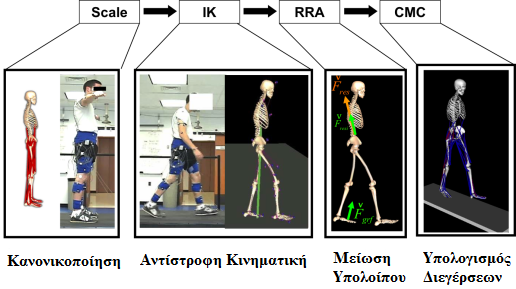
\includegraphics[width=0.7\textwidth, keepaspectratio]{fig/ik-to-excitation.png}
    \caption{Τυπική ροή υπολογισμού των μυϊκών διεγέρσεων\protect\footnotemark}
    \label{fig:ik-to-excitation}
\end{figure}
\footnotetext{Εικόνα από την ιστοσελίδα \eng{\url{http://simtk-confluence.stanford.edu:8080/display/OpenSim/Overview+of+the+OpenSim+Workflow}}}

Μια τυπική ροή ώστε να φτάσουμε σε νευρικό επίπεδο διεγέρσεων περιγράφεται από την εικόνα \ref{fig:ik-to-excitation}. Η διεργασία πριν τον υπολογισμό των μυϊκών διεγέρσεων ονομάζεται αλγόριθμος υπολειμματικής μείωσης (\eng{residual redaction algorithm}) και μπορεί να παραληφθεί, αλλά γενικά βελτιώνει το αποτέλεσμα.

%%%%%%%%%%%%%%%%%%%%%%%%%%%%%%%%%%%%%%%%%%%%%%%%%%%%%%%%%%%%%%%%%%%%%%%%%%%%%%%%
\subsection{Εκτίμηση των Μυϊκών Δυνάμεων}

Όπως αναφέραμε η διαδικασία προσδιορισμού των μυϊκών δυνάμεων βασίζεται στην βελτιστοποίηση. Ξέρουμε για κάθε άρθρωση την χρονική ακολουθία των ροπών από την αντίστροφη δυναμική. Επίσης ξέρουμε από την γεωμετρία του μοντέλου την τοποθεσία κάθε μυ σε ποια άρθρωση συνεισφέρει έργο. Σε μια άρθρωση μπορούν να συνεισφέρουν έργο παραπάνω από έναν μυ. Ένα κριτήριο βελτιστοποίησης μπορεί να είναι το να ελαχιστοποιηθεί η ενέργεια ώστε να παραχθεί η δοσμένη κίνηση. Το κριτήριο αυτό, ανάλογα και την εφαρμογή, είναι λογικό αφού για κάθε κίνηση προσπαθούμε να καταβάλουμε όσον το δυνατόν λιγότερη προσπάθεια στην πράξη, όταν βέβαια δεν υπάρχει κάποια σοβαρή ασθένεια. Συμπερασματικά, το πρόβλημα μπορεί να διατυπωθεί μαθηματικά ως εξής.\\

\begin{equation}
    \begin{gathered}
        \underset{a}{\text{\eng{minimize}}} \sum_{i=1}^{N} a_{i}^{p} \\
        \text{\eng{s.t.}} \quad
        \sum_{i=1}^{N} (a_{i} \cdot f(f^{o}_{i}, l_{i}, v_{i})) \cdot  R_{ij} = \tau_{j}, \quad \forall j
    \end{gathered}
    \label{equ:static-optimization}
\end{equation}

Όπου $a_i$ είναι το επίπεδο ενεργοποίησης του μυ $i$, η συνάρτηση $f(f^{o}_{i}, l_{i}, v_{i})$ είναι η δύναμη που παράγει ο μυς χωρίς να λάβουμε υπόψη τον τένοντα με $f^{o}_{i}, l_{i}, v_{i}$ να είναι η μέγιστη ισομετρική δύναμη, το μήκος και η ταχύτητα του μυ αντίστοιχα. Το $R_{ij}$ είναι η μυϊκή ροπή αδράνειας και το $\tau_{j}$ είναι η ροπή στην άρθρωση $j$.

%%%%%%%%%%%%%%%%%%%%%%%%%%%%%%%%%%%%%%%%%%%%%%%%%%%%%%%%%%%%%%%%%%%%%%%%%%%%%%%%
\subsection{Προσδιορισμός των Μυϊκών Διεγέρσεων}

Η διαδικασία προσδιορισμού των διεγέρσεων είναι σχετικά πολύπλοκη και συνδυάζει πολλές μεθόδους μαζί και για διευκόλυνση θα περιγράψουμε την διαδικασία ιεραρχικά. Η μέθοδος αυτή παίρνει σαν ορίσματα τις πειραματικές τροχαίες των αρθρώσεων, μαζί μαι τις δύο πρώτες παραγώγους και τις εξωτερικές δυνάμεις. Το αποτέλεσμα είναι οι διεγέρσεις για κάθε μυ σε κάθε χρονική στιγμή.

Όπως περιγράφεται και στην εικόνα \ref{fig:cmc-diagram} βλέπουμε ότι όλη η διαδικασία είναι κλειστού βρόγχους, που σημαίνει ότι κάθε χρονική στιγμή το σύστημα τροφοδοτείται κατάλληλα, ώστε η παραγόμενη κίνηση να είναι όσο το δυνατόν ταυτόσημη με την πειραματική. Χρησιμοποιείται \eng{PD} ελεγκτή, όπου οι σταθερές επιλέγονται ώστε να πετύχουμε κρίσιμη απόσβεση ($\overrightarrow{k}_v = 2 \cdot \sqrt{\overrightarrow{k}_p}$). Επίσης βλέπουμε ότι η επιθυμητή επιτάχυνσή $\ddot{\overrightarrow{q}}^{*}$ υπολογίζεται για μελλοντική τιμή $t + \tau $. Αυτό γιατί οι μύες έχουν μια καθυστέρηση, οπότε η διέγερση θα πρέπει να προηγείται κατά μια μικρή χρονική στιγμή (συνήθως $\tau = 0.01$). Έπειτα εκτελείται στατική βελτιστοποίηση για να υπολογιστούν οι απαιτούμενες διεγέρσεις που στην συνέχεια τροφοδοτούνται στο σύστημα με την βοήθεια της ορθής δυναμικής, η οποία θα παράξει την κίνηση με βάση αυτών.

\begin{figure}[H]
    \centering
    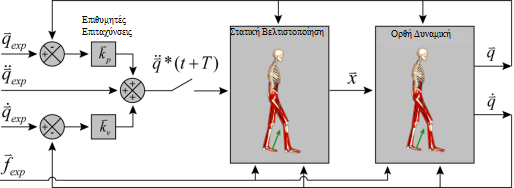
\includegraphics[width=0.8\textwidth, keepaspectratio]{fig/cmc-diagram.png}
    \caption{Διάγραμμα της διαδικασίας υπολογισμού μυϊκών διεγέρσεων \cite{thelen06}}
    \label{fig:cmc-diagram}
\end{figure}

Η διαδικασία είναι σύνθετη και στην πράξη έχει μεγάλες καθυστερήσεις, που ανάλογα από τον υπολογιστή μπορεί να κυμαίνονται από 15 λεπτά για έναν σύγχρονο υπολογιστή έως και πάνω από μισή ώρα για πιο παλιούς ώστε να παραχθεί ένα αποτέλεσμα διάρκειας μισού λεπτού. Επίσης η διαδικασία μπορεί να διακοπεί αν δεν πληρούνται τα επιτρεπτά όρια ανοχής σε σφάλματα. Συχνά για την βελτίωση της διαδικασίας εισάγονται επιπλέον εφεδρικοί κινητήρες στις αρθρώσεις για να παρέχουν την απαραίτητη ροπή, ώστε να παραχθεί η κίνηση, καθώς οι μύες μπορεί να μην είναι σε θέση να οδηγήσουν το σύστημα στην επιθυμητή κατάσταση. Το τελευταίο οφείλεται συνήθως σε απλοποιήσεις στο μοντέλο, μειώνοντας τους μύες με αποτέλεσμα να μην επαρκεί η κινητική τους δύναμη. Επειδή συνήθως δεν μπορούν να αποφευχθούν οι εφεδρικοί κινητήρες, αν δούμε ότι η προσομοίωση τρέχει ήμαστε σε θέση να ελαττώσουμε την επιρροή τους και να βασιστούμε στους μύες του μοντέλου.


